\subsection{EDDenseNet}
The model is the following:
\begin{figure}[H]
    \centering
    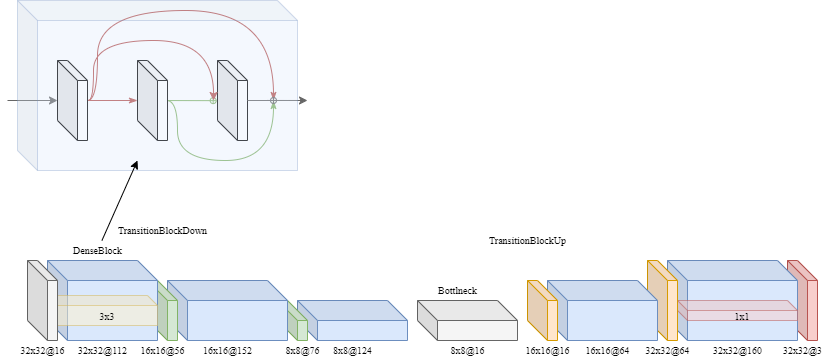
\includegraphics[scale=0.5]{subsections/densenet/densenet.png}
\end{figure}

The DenseNet\cite{densenet} architecture improve the ResNet skip connections allowing the concatenation instead of doing the sum: each DenseBlock contains layers whose input is the concatenation of all previous layers' channels output allowing \textit{feature reuse} which increase the performance of the network because allow a better flow of the information on the network and at the same time allow to have more compact network.
Each DenseBlock contains bottleneck layer before each 3x3 convolution in order to reduce the number of parameters.

After each DenseBlock, a TransitionBlock is inserted which downsamples the output of a dense block.

In the paper the DenseNet-121 has a growth rate of 32 and the number of blocks are [6,12,24,16]  

The model implemented has different characteristics:
\begin{itemize}
    \item There are TransitionBlocks which upsample the output of a DenseBlock in order to mimic the Encoder-Decoder architecture.
    \item The growth rate is 16 and the number of layers for the encoder are [6, 6, 3] and for the decoder [3, 6].
    \item A bottleneck layer is used for reducing the number of channels at the end of the encoder (thus reducing the number of parameters): for instance without the bottleneck layer the amount of parameters would be $124*3*3*124+124=138384$, instead with the bottleneck layer is $124*3*3*16+16 = 17872$ (so with bottleneck layer using a large growth rate and more layers would reduce a lot the parameters therefore reducing also the training time)
    \item With respect to the original paper the downsampling and upsampling is done respectively using Conv2D and Conv2DTranspose in order to "learn" the transformation instead of using MaxPooling and UpSampling leading to a loss of information.
    \item The last layer is a Conv2DTranspose which "learn" to decode the output.
\end{itemize}
\subsection{Training}
The network was trained with Adam\cite{adam} with default parameters and MSE as loss function.
The network converged within 22 epochs with early stopping equals to 5.
\begin{figure}[H]
    \centering
    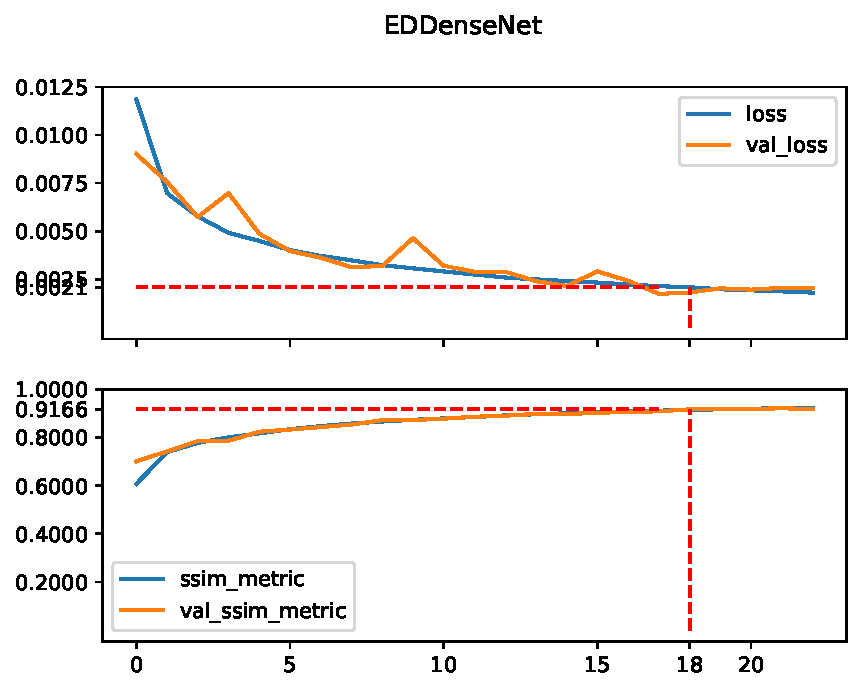
\includegraphics[height=0.4\textheight,keepaspectratio]{subsections/densenet/plot_history_EDDenseNet.pdf}
    \caption{Training information of EDDenseNet.}
\end{figure}        

\subsection{Results}
The evaluation of the network is the following:
\begin{center}
    \small
    \begin{tabularx}{165pt}{c|ccc}
        \centering
        kernel type & MSE & PSNR & SSIM \\
        \hline
        gaussian & 0.0021 & 27.62 & 0.90
    \end{tabularx}        
\end{center}

My implementation (the encoder) is not so deep as the one implemented by researchers, nevertheless the results are quite good.

\begin{figure}[H]
    \centering
    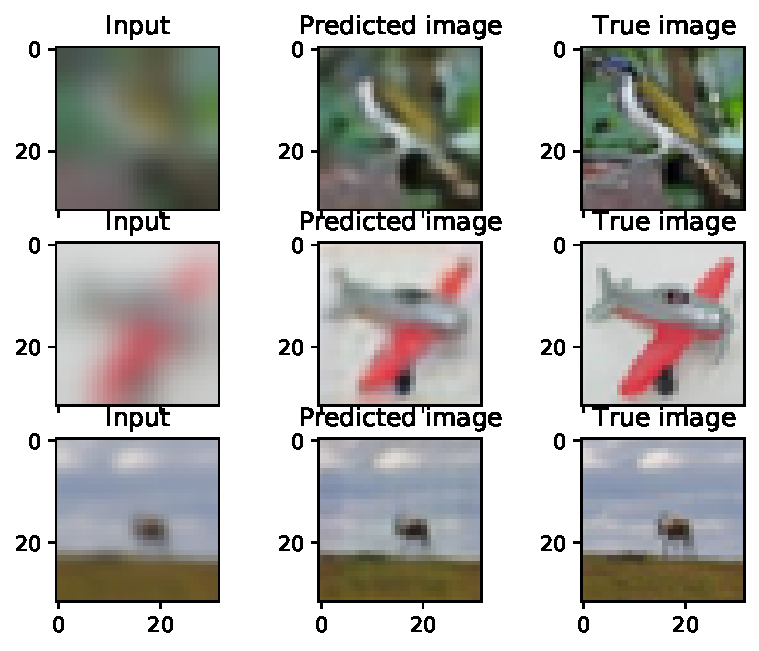
\includegraphics[height=0.5\textheight,keepaspectratio]{subsections/densenet/test.pdf}
    \caption{Test image generated by EDDenseNet.}
\end{figure}

Looking at the images I can assert that the network is able to restore fine details from the blurred image even when they are not visible (i.e. the cockpit of the plane or the details on the chest of the bird).



